\documentclass{beamer}
\usepackage[utf8]{inputenc}
\usepackage{tikz}
\usetikzlibrary{positioning}
\usetheme{Madrid}
\usepackage{listings}
\usepackage{booktabs}
\usepackage[backend=biber,
style=alphabetic-verb]{biblatex}
\usecolortheme{default}
\usepackage{caption}
\usepackage{subcaption}
\usepackage{tcolorbox}
\usepackage{svg}
\usepackage{xcolor}
\usepackage{algorithm2e}
% Code styling
\definecolor{codegreen}{rgb}{0,0.6,0}
\definecolor{codegray}{rgb}{0.5,0.5,0.5}
\definecolor{codepurple}{rgb}{0.58,0,0.82}
\definecolor{backcolour}{rgb}{0.95,0.95,0.92}

\lstdefinestyle{mystyle}{
    backgroundcolor=\color{backcolour},   
    commentstyle=\color{codegreen},
    keywordstyle=\color{magenta},
    numberstyle=\color{codegray},
    stringstyle=\color{codepurple},
    basicstyle=\ttfamily\tiny,
    breakatwhitespace=false,         
    breaklines=True,                 
    captionpos=b,                    
    keepspaces=true,                 
    numbers=none,                    
    showspaces=false,                
    showstringspaces=false,
    showtabs=false,                  
    tabsize=2
}

\lstset{style=mystyle}
%------------------------------------------------------------
%This block of code defines the information to appear in the
%Title page
\addbibresource{bibliographie.bib}
\title %optional
[Interpretable RL]{Interpretability, Decision Trees, and Sequential Decision Making}

\author[Hector Kohler] % (optional)
{Hector Kohler}

\institute[Univ. Lille] % (optional)
{
  Supervised by Dr. Riad Akrour (HdR) and Prof. Philippe Preux (HdR)\\
  Universit\'e de Lille, CNRS, Inria, UMR CRIStAL 9189, France
}

\begin{document}

\frame{\titlepage}


%% -----------------------INTRO-----------------------
\begin{frame}{Sequential decision making (SDM)}
\begin{figure}
    \centering
    \begin{tikzpicture}[
        node distance=2.5cm,
        auto,
        thick,
        state/.style={circle, draw, fill=blue!20, minimum size=1.5cm, text centered},
        environment/.style={rectangle, draw, dashed, fill=blue!10, rounded corners, minimum width=4cm, minimum height=2cm, text centered},
        agent/.style={rectangle, draw, fill=orange!20, rounded corners, minimum width=2cm, minimum height=1.5cm, text centered},
        robot/.style={rectangle, draw, fill=green!20, rounded corners, minimum width=2cm, minimum height=1.5cm, text centered},
        decision_box/.style={rectangle, draw, dashed, fill=gray!10, minimum width=7.5cm, minimum height=3cm, text centered},
        arrow/.style={->, thick, bend left=15},
        arrow_decision/.style={->, dashed, bend left=15}
    ]
        
        % Decision Making Box
        \node[decision_box] (decision_box) at (0.3,3.4) {};
        \node at (0.3,4.5) {\small{Decision Making}};
        
        % Robot (AI)
        \node[robot] (robot) at (-2.1,3.2) {
            \begin{minipage}{1.5cm}
                \centering
                \includesvg[width=0.4cm]{../images/images_intro/robot-svgrepo-com.svg}\\
                \small{Policy}
            \end{minipage}
        };
        
        % Doctor
        \node[agent] (doctor) at (2.5,3.2) {
            \begin{minipage}{1.5cm}
                \centering
                \includesvg[width=0.4cm]{../images/images_intro/doctor-with-stethoscope-svgrepo-com.svg}\\
                \small{Doctor}
            \end{minipage}
        };
        
        % Environment (Patient)
        \node[environment] (environment) at (0,-0.5) {
            \begin{minipage}{2cm}
                \centering
                \includesvg[width=0.8cm]{../images/images_intro/patient-4.svg}\\
                \small{Cancer patient}
            \end{minipage}
        };
        
        % Arrows
        \draw[arrow] (environment) to[bend left=30] node[left] {
            \begin{minipage}{2cm}
                \centering
                \includesvg[width=0.4cm]{../images/images_intro/patient-clipboard-svgrepo-com.svg}\\
                \small{Updated health status}
            \end{minipage}
        } (robot);
        \draw[arrow_decision] (robot) to node[above] {\small{Recommends}} (doctor);
        \draw[arrow_decision] (doctor) to node[below] {\small{Interprets}} (robot);

        \draw[arrow] (doctor) to[bend left=30] node[right] {
            \begin{minipage}{1.5cm}
                \centering
                \includesvg[width=0.5cm]{../images/images_intro/syringe-svgrepo-com.svg}\\
                \small{Administer chemotherapy}
            \end{minipage}
        } (environment);
        
    \end{tikzpicture}
    \caption{Sequential decision making in cancer treatment.}
\end{figure}
\end{frame}

\begin{frame}{Machine learning (ML) of policies for SDM}
\begin{figure}
\hspace{-1.3cm}
        \begin{tikzpicture}[
            node distance=2.5cm,
            auto,
            thick,
            state/.style={circle, draw, fill=blue!20, minimum size=1.5cm, text centered},
            environment/.style={rectangle, draw, dashed, fill=blue!10, rounded corners, minimum width=4cm, minimum height=2cm, text centered},
            agent/.style={rectangle, draw, fill=orange!20, rounded corners, minimum width=2cm, minimum height=1.5cm, text centered},
            robot/.style={rectangle, draw, fill=black!20, rounded corners, minimum width=2cm, minimum height=1.5cm, text centered},
            ml/.style={circle, draw, fill=purple!20, minimum width=1cm, minimum height=1cm, text centered},
            decision_box/.style={rectangle, draw, dashed, fill=gray!10, minimum width=7.5cm, minimum height=3cm, text centered},
            arrow/.style={->, thick, bend left=15},
            arrow_decision/.style={->, dashed, bend left=15},
            scale=0.98
        ]
            
            % Decision Making Box
            \node[decision_box] (decision_box) at (0.3,3.4) {};
            \node at (0.3,4.5) {\small{Decision Making}};
            
            % Robot (AI)
            \node[robot] (robot) at (-2.1,3.2) {
                \begin{minipage}{1.5cm}
                    \centering
                    \includesvg[width=0.4cm]{../images/images_intro/network-mapping-svgrepo-com.svg}\\
                    \small{Neural network}
                \end{minipage}
            };
            
            % Doctor
            \node[agent] (doctor) at (2.5,3.2) {
                \begin{minipage}{1.5cm}
                    \centering
                    \includesvg[width=0.4cm]{../images/images_intro/doctor-with-stethoscope-svgrepo-com.svg}\\
                    \small{Doctor}
                \end{minipage}
            };
            
            % Machine Learning component
            \node[ml] (ml) at (-6,3) {
                \begin{minipage}{1cm}
                    \centering
                    \includesvg[width=0.4cm]{../images/images_intro/gear-file-svgrepo-com.svg}\\
                    \small{ML}
                \end{minipage}
            };
            
            % Environment (Patient)
            \node[environment] (environment) at (0,-0.5) {
                \begin{minipage}{2cm}
                    \centering
                    \includesvg[width=0.8cm]{../images/images_intro/patient-4.svg}\\
                    \small{Cancer patient}
                \end{minipage}
            };
            
            % Arrows
            \draw[arrow] (environment) to[bend left=30] node[left] {
                \begin{minipage}{2cm}
                    \centering
                    \includesvg[width=0.5cm]{../images/images_intro/patient-clipboard-svgrepo-com.svg}\\
                    \small{Updated health status}
                \end{minipage}
            } (robot);
            \draw[arrow_decision] (robot) to node[above] {\small{Recommends}} (doctor);
            \draw[arrow_decision, red] (doctor) to node[below] {\small{Cannot interpret}} (robot);
            
        \draw[arrow] (doctor) to[bend left=30] node[right] {
                \begin{minipage}{1.5cm}
                    \centering
                    \includesvg[width=0.5cm]{../images/images_intro/syringe-svgrepo-com.svg}\\
                \small{Administer chemotherapy}
                \end{minipage}
            } (environment);
            
            % ML learning arrows
            \draw[arrow] (environment) to[bend left=40] node[left] {
                \begin{minipage}{2cm}
                    \centering
                    \includesvg[width=0.5cm]{../images/images_intro/patient-clipboard-svgrepo-com.svg}\\
                    \small{Treatment outcomes}
                \end{minipage}
            } (ml);
            \draw[arrow] (ml) to[bend left=20] node[above] {
                \begin{minipage}{1.5cm}
                    \centering
                    \small{Updates policy}
                \end{minipage}
            } (robot);
            
        \end{tikzpicture}
        \caption{Machine learning of neural networks has many recent successes but neural networks are black-box.}
    \end{figure}
\end{frame}

% \begin{frame}{Interpretable machine learning for sequential decision making}
% \begin{figure}
% \hspace{-1.3cm}
%     \begin{tikzpicture}[
%             node distance=2.5cm,
%             auto,
%             thick,
%             state/.style={circle, draw, fill=blue!20, minimum size=1.5cm, text centered},
%             environment/.style={rectangle, draw, dashed, fill=blue!10, rounded corners, minimum width=4cm, minimum height=2cm, text centered},
%             agent/.style={rectangle, draw, fill=orange!20, rounded corners, minimum width=2cm, minimum height=1.5cm, text centered},
%             robot/.style={rectangle, draw, fill=green!20, rounded corners, minimum width=2cm, minimum height=1.5cm, text centered},
%             ml/.style={circle, draw, fill=purple!20, minimum width=1cm, minimum height=1cm, text centered},
%             decision_box/.style={rectangle, draw, dashed, fill=gray!10, minimum width=7.5cm, minimum height=3cm, text centered},
%             arrow/.style={->, thick, bend left=15},
%             arrow_decision/.style={->, dashed, bend left=15},
%             scale=0.98
%         ]
            
%             % Decision Making Box
%             \node[decision_box] (decision_box) at (0.3,3.4) {};
%             \node at (0.3,4.5) {\small{Decision Making}};
            
%             % Robot (AI)
%             \node[robot] (robot) at (-2.1,3.2) {
%                 \begin{minipage}{1.5cm}
%                     \centering
%                     \includesvg[width=0.4cm]{../images/images_intro/decision-tree-svgrepo-com.svg}\\
%                     \small{Decision tree}
%                 \end{minipage}
%             };
            
%             % Doctor
%             \node[agent] (doctor) at (2.5,3.2) {
%                 \begin{minipage}{1.5cm}
%                     \centering
%                     \includesvg[width=0.4cm]{../images/images_intro/doctor-with-stethoscope-svgrepo-com.svg}\\
%                     \small{Doctor}
%                 \end{minipage}
%             };
            
%             % Machine Learning component
%             % Machine Learning component
%             \node[ml] (ml) at (-6,3) {
%                 \begin{minipage}{1cm}
%                     \centering
%                     \includesvg[width=0.4cm]{../images/images_intro/gear-file-svgrepo-com.svg}\\
%                     \small{ML}
%                 \end{minipage}
%             };
            
%             % Environment (Patient)
%             \node[environment] (environment) at (0,-0.5) {
%                 \begin{minipage}{2cm}
%                     \centering
%                     \includesvg[width=0.8cm]{../images/images_intro/patient-4.svg}\\
%                     \small{Cancer patient}
%                 \end{minipage}
%             };
            
%             % Arrows
%             \draw[arrow] (environment) to[bend left=30] node[left] {
%                 \begin{minipage}{2cm}
%                     \centering
%                     \includesvg[width=0.5cm]{../images/images_intro/patient-clipboard-svgrepo-com.svg}\\
%                     \small{Updated health status}
%                 \end{minipage}
%             } (robot);
%             \draw[arrow_decision] (robot) to node[above] {\small{Recommends}} (doctor);
%             \draw[arrow_decision, green] (doctor) to node[below] {\small{Can interpret}} (robot);
            
%         \draw[arrow] (doctor) to[bend left=30] node[right] {
%                 \begin{minipage}{1.5cm}
%                     \centering
%                     \includesvg[width=0.5cm]{../images/images_intro/syringe-svgrepo-com.svg}\\
%                 \small{Administer chemotherapy}
%                 \end{minipage}
%             } (environment);
            
%             % ML learning arrows
%             \draw[arrow] (environment) to[bend left=40] node[left] {
%                 \begin{minipage}{2cm}
%                     \centering
%                     \includesvg[width=0.5cm]{../images/images_intro/patient-clipboard-svgrepo-com.svg}\\
%                     \small{Treatment outcomes}
%                 \end{minipage}
%             } (ml);
%             \draw[arrow] (ml) to[bend left=20] node[above] {
%                 \begin{minipage}{1.5cm}
%                     \centering
%                     \small{Updates policy}
%                 \end{minipage}
%             } (robot);
            
%         \end{tikzpicture}
%         \caption{Some machine learning algorithms can learn interpretable policies, e.g. decision trees.}
%         \label{fig:cancer-treatment-comparison}
%     \end{figure}
% \end{frame}

\begin{frame}{Research direction}
    \textbf{\large How to \textcolor{blue}{learn} \textcolor{green}{interpretable} policies for \textcolor{orange}{sequential decision making}?}
\end{frame}
%% ------------- FORMALISM ------------------------------
\begin{frame}{Policy interpretability}
\begin{figure}
    \centering
    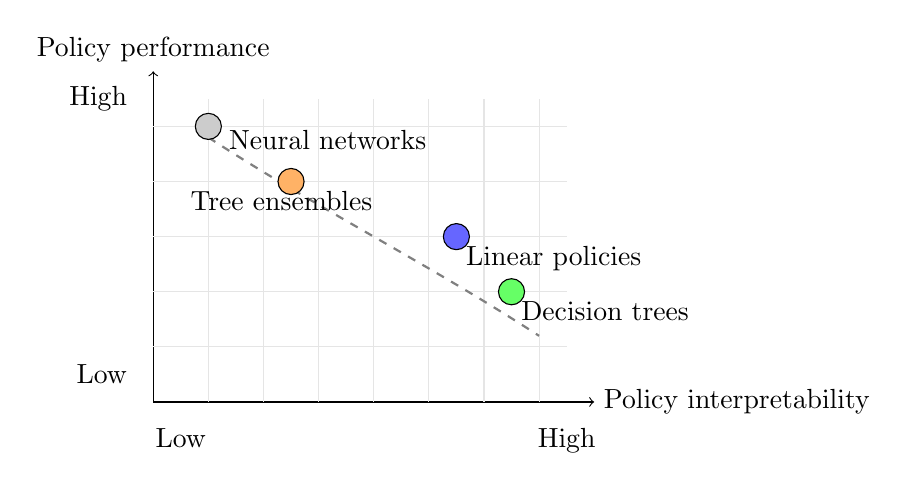
\begin{tikzpicture}[scale=0.7]
        % Define the axes
        \draw[->] (0,0) -- (8,0) node[right] {Policy interpretability};
        \draw[->] (0,0) -- (0,6) node[above] {Policy performance};
        
        % Add axis labels at the ends
        \node[below] at (0.5,-0.3) {Low};
        \node[below] at (7.5,-0.3) {High};
        \node[left] at (-0.3,0.5) {Low};
        \node[left] at (-0.3,5.5) {High};
        
        % Add grid lines (optional, subtle)
        \foreach \x in {1,2,...,7}
            \draw[gray!20] (\x,0) -- (\x,5.5);
        \foreach \y in {1,2,...,5}
            \draw[gray!20] (0,\y) -- (7.5,\y);
        
        % Add a general trend line (optional)
        \draw[dashed, thick, gray] (1,4.8) .. controls (3,3.5) and (5,2.5) .. (7,1.2);
        
        % Position different model types
        % Deep Neural Networks (high performance, low interpretability)
        \node[circle, fill=black!20, draw, minimum size=8pt] at (1,5) {};
        \node[below right] at (1.2,5.1) {Neural networks};
        
        % Ensemble Methods (medium-high performance, low-medium interpretability)
        \node[circle, fill=orange!60, draw, minimum size=8pt] at (2.5,4) {};
        \node[below right] at (0.5,4) {Tree ensembles};
        
        % Linear Models (medium performance, high interpretability)
        \node[circle, fill=blue!60, draw, minimum size=8pt] at (5.5,3) {};
        \node[below right] at (5.5,3) {Linear policies};
        
        % Decision Trees (medium-low performance, high interpretability)
        \node[circle, fill=green!60, draw, minimum size=8pt] at (6.5,2) {};
        \node[below right] at (6.5,2) {Decision trees};
        
    \end{tikzpicture}
    \caption{\textbf{Heuristic} interpretability-performance trade-offs of different policy classes. Interpretability is often presented in opposition to performances.}
\end{figure}
\end{frame}

\begin{frame}{Decision trees}
\begin{figure}
    \centering
    \scalebox{0.8}{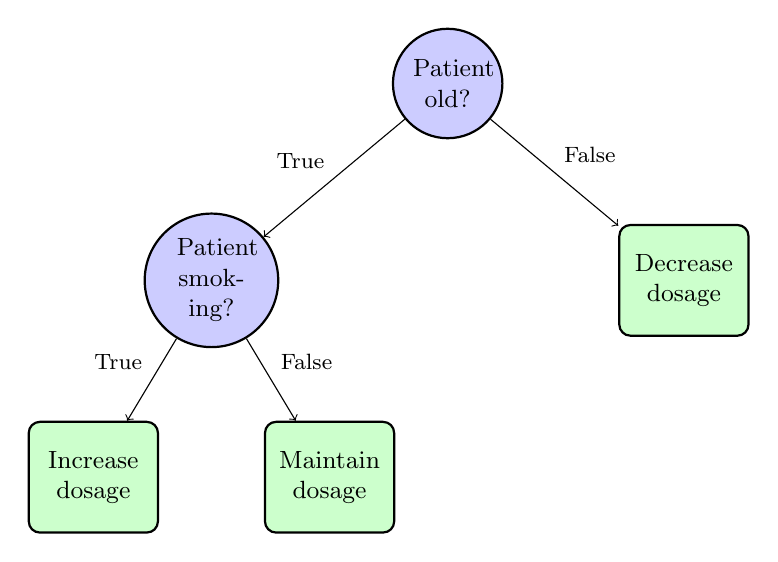
\begin{tikzpicture}[
        scale=1.0,
        decision/.style={circle, draw, thick, fill=blue!20, text width=2.5em, text centered, minimum height=2.5em, font=\small},
        leaf/.style={rectangle, draw, thick, fill=green!20, text width=4em, text centered, rounded corners, minimum height=4em, font=\small},
        edge_label/.style={font=\footnotesize, midway}
    ]
        % Root decision node
        \node[decision] (root) at (0,0) {Patient old?};
        
        % Second level nodes
        \node[decision] (left_decision) at (-3, -2.5) {Patient smoking?};
        \node[leaf] (right_leaf) at (3, -2.5) {Decrease dosage};
        
        % Third level nodes (leaves)
        \node[leaf] (left_left) at (-4.5, -5) {Increase dosage};
        \node[leaf] (left_right) at (-1.5, -5) {Maintain dosage};
        
        % Connections with labels
        \draw[->] (root) -- (left_decision) node[edge_label, above left] {True};
        \draw[->] (root) -- (right_leaf) node[edge_label, above right] {False};
        \draw[->] (left_decision) -- (left_left) node[edge_label, above left] {True};
        \draw[->] (left_decision) -- (left_right) node[edge_label, above right] {False};
        
        % Add labels for components
        % \node[font=\footnotesize, text=gray] at (0, 0.8) {Root node with test $t_1(x_i)$};
        % \node[font=\footnotesize, text=gray] at (-6, -2.5) {Internal node with test $t_2(x_i)$};
        % \node[font=\footnotesize, text=gray] at (-3, -5.8) {Leaf nodes with predictions};
        
    \end{tikzpicture}}
    \caption{A generic decision tree of depth $D=2$. Easy to learn in the supervised learning setting: Classification And Regression Trees (CART, \cite{breiman1984classification}), Optimal Classification Trees (OCT, \cite{oct}). What about sequential decision making?}
\end{figure}
\end{frame}

\begin{frame}{Markov decision processes}
\begin{figure}
    \centering
    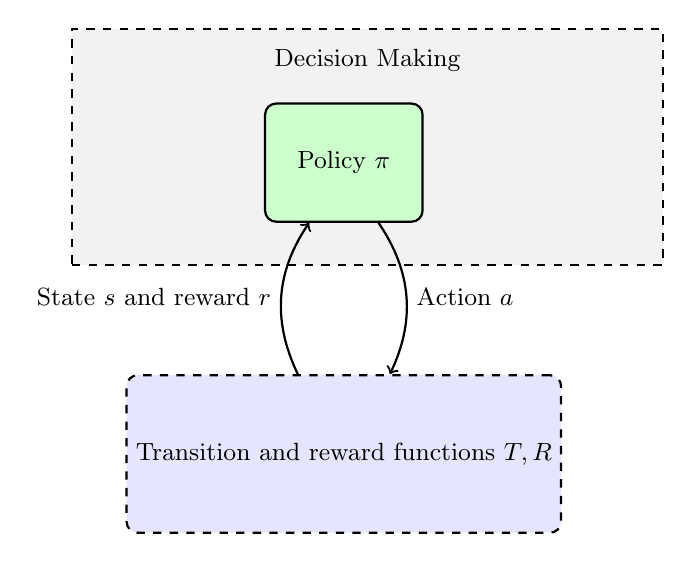
\begin{tikzpicture}[
        node distance=2.5cm,
        auto,
        thick,
        state/.style={circle, draw, fill=blue!20, minimum size=1.5cm, text centered},
        environment/.style={rectangle, draw, dashed, fill=blue!10, rounded corners, minimum width=4cm, minimum height=2cm, text centered},
        agent/.style={rectangle, draw, fill=orange!20, rounded corners, minimum width=2cm, minimum height=1.5cm, text centered},
        robot/.style={rectangle, draw, fill=green!20, rounded corners, minimum width=2cm, minimum height=1.5cm, text centered},
        decision_box/.style={rectangle, draw, dashed, fill=gray!10, minimum width=7.5cm, minimum height=3cm, text centered},
        arrow/.style={->, thick, bend left=15},
        arrow_decision/.style={->, dashed, bend left=15}
    ]
        
        % Decision Making Box
        \node[decision_box] (decision_box) at (0.3,3.4) {};
        \node at (0.3,4.5) {\small{Decision Making}};
        
        % Robot (AI)
        \node[robot] (robot) at (0,3.2) {\small{Policy $\pi$}};
        
        
        % Environment (Patient)
        \node[environment] (environment) at (0,-0.5) {\small{Transition and reward functions $T, R$}};
        
        % Arrows
        \draw[arrow] (environment) to[bend left=30] node[left] {\small{State $\boldsymbol{s}$ and reward $r$}} (robot);
        \draw[arrow] (robot) to[bend left=30] node[right] {\small{Action $a$}} (environment);
        
    \end{tikzpicture}
    \caption{Markov decision process (\cite{puterman}).}
\end{figure}
\end{frame}

\begin{frame}{Reinforcement learning (RL) objective}
\begin{itemize}
    \item Given an MDP $\mathcal{M}=\langle S, A, R, T, T_0 \rangle$, the goal of RL (\cite{sutton}) for SDM is to find a policy, $\pi: S \rightarrow A$ that maximizes the expected discounted sum of rewards:
    \begin{align}
        J(\pi) &= \mathbb{E}\left[\sum_{t=0}^{\infty} \gamma^t R(s_t, a_t) \mid s_0 \sim T_0, a_t = \pi(s_t), s_{t+1} \sim T(s_t, a_t)\right]
    \end{align}
    where $0< \gamma\leq 1$ is the discount factor that controls the trade-off between immediate and future rewards.
    \item Value iteration, Q-learning, Sarsa, Deep Q Networks, Proximal Policy Optimization, \dots (\cite{Bellman,sutton,dqn,ppo})
\end{itemize}
\end{frame}

% ------------ Example -------------------------
\begin{frame}{Grid world MDP}
\begin{figure}
    \centering
    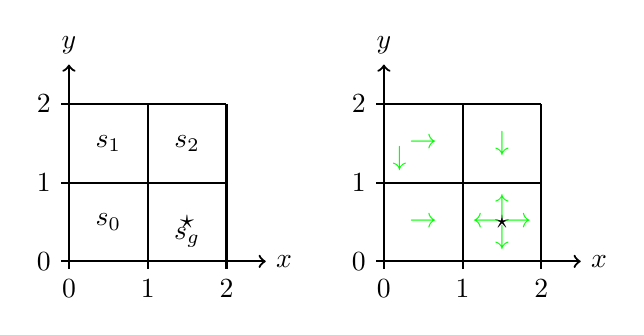
\begin{tikzpicture}
        \tikzstyle{grid}=[draw, thick, fill=gray!10]
        
        % Draw grid
        \draw[grid] (0,0) grid (2,2);
        
        % Add axes
        \draw[thick, ->] (0,0) -- (2.5,0) node[right] {$x$};
        \draw[thick, ->] (0,0) -- (0,2.5) node[above] {$y$};
        
        % Add tick marks and labels
        \foreach \x in {0,1,2} {
            \draw[thick] (\x,0) -- (\x,-0.1) node[below] {$\x$};
        }
        \foreach \y in {0,1,2} {
            \draw[thick] (0,\y) -- (-0.1,\y) node[left] {$\y$};
        }
        
        % Add state labels clockwise from bottom left
        \node at (0.5,0.5) {$s_0$};
        \node at (1.5,0.5) {$\star$};
        \node at (1.5,0.3) {$s_g$};
        \node at (1.5,1.5) {$s_2$};
        \node at (0.5,1.5) {$s_1$};


        % Draw grid
        \draw[grid] (4,0) grid (6,2);
        
        % Add axes
        \draw[thick, ->] (4,0) -- (6.5,0) node[right] {$x$};
        \draw[thick, ->] (4,0) -- (4,2.5) node[above] {$y$};
        
        % Add tick marks and labels
        \draw[thick] (4,0) -- (4,-0.1) node[below] {$0$};
        \draw[thick] (5,0) -- (5,-0.1) node[below] {$1$};
        \draw[thick] (6,0) -- (6,-0.1) node[below] {$2$};
        

        \foreach \y in {0,1,2} {
            \draw[thick] (4,\y) -- (3.9,\y) node[left] {$\y$};
        }
        
        % Add state labels clockwise from bottom left
        \node at (4.5,0.5) {{\color{green} $\rightarrow$}};
        \node at (5.5,0.5) {$\star$};
        \node at (5.5,0.7) {{\color{green} $\uparrow$}};
        \node at (5.5,0.3) {{\color{green} $\downarrow$}};
        \node at (5.7,0.5) {{\color{green} $\rightarrow$}};
        \node at (5.3,0.5) {{\color{green} $\leftarrow$}};
        \node at (5.5,1.5) {{\color{green} $\downarrow$}};
        \node at (4.2,1.3) {{\color{green} $\downarrow$}};
        \node at (4.5,1.5) {{\color{green} $\rightarrow$}};
    \end{tikzpicture}
    \caption{A grid world MDP and optimal actions w.r.t. the RL objective.}
    \end{figure}
\end{frame}

\begin{frame}{Example: a decision tree policy for the grid world MDP}
\begin{figure}
    \centering
    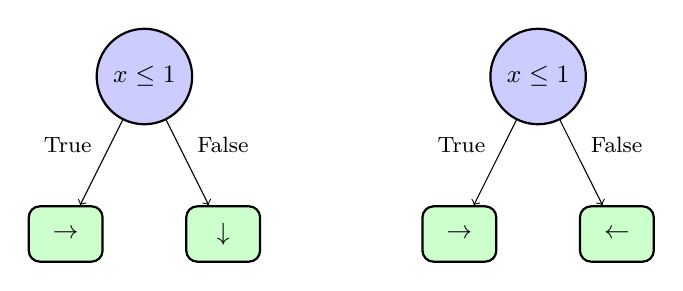
\begin{tikzpicture}[
        decision/.style={circle, draw, thick, fill=blue!20, text width=2.5em, text centered, minimum height=2.5em, font=\small},
        leaf/.style={rectangle, draw, thick, fill=green!20, text width=2em, text centered, rounded corners, minimum height=2em, font=\small},
        edge_label/.style={font=\footnotesize, midway}
    ]
        % Tree 4: if x <= 0.5 move right else move left
        \node[decision] (tree4_root) at (10,2) {$x \leq 1$};
        \node[leaf] (tree4_right) at (9,0) {$\rightarrow$};
        \node[leaf] (tree4_left) at (11,0) {$\leftarrow$};
        \draw[->] (tree4_root) -- (tree4_right) node[edge_label, above left] {True};
        \draw[->] (tree4_root) -- (tree4_left) node[edge_label, above right] {False};
        \tikzstyle{grid}=[draw, thick, fill=gray!10]


        % Tree 4: if x <= 0.5 move right else move left
        \node[decision] (tree5_root) at (5,2) {$x \leq 1$};
        \node[leaf] (tree5_right) at (4,0) {$\rightarrow$};
        \node[leaf] (tree5_left) at (6,0) {$\downarrow$};
        \draw[->] (tree5_root) -- (tree5_right) node[edge_label, above left] {True};
        \draw[->] (tree5_root) -- (tree5_left) node[edge_label, above right] {False};
        \tikzstyle{grid}=[draw, thick, fill=gray!10]

    \end{tikzpicture}
    \caption{Left, an optimal depth-1 decision tree policy. On the right, a sub-optimal depth-1 decision tree policy.}
    \end{figure}
\end{frame}

% -------------- Existing works --------------
% \begin{frame}{Two ways to get interpretable policies for SDM}
% \begin{figure}
%     \centering
%     \scalebox{0.82}{\begin{tikzpicture}[
%         node distance=2cm,
%         scale=1,
%         auto,
%         thick,
%         rl/.style={circle, draw, fill=purple!20, minimum width=1.5cm, minimum height=0.8cm, text centered},
%         nn/.style={rectangle, draw, fill=black!20, rounded corners, minimum width=1.5cm, minimum height=1cm, text centered},
%         sl/.style={circle, draw, fill=blue!20, minimum width=1.5cm, minimum height=0.8cm, text centered},
%         dt/.style={rectangle, draw, fill=green!20, rounded corners, minimum width=1.5cm, minimum height=1cm, text centered},
%         arrow/.style={->, thick},
%         label/.style={font=\tiny, above},
%         method_box/.style={rectangle, draw, dashed, minimum width=5cm, minimum height=3cm, text centered},
%         method_box_indirect/.style={rectangle, draw, dashed, minimum width=9.5cm, minimum height=3cm, text centered}
%     ]
        
%         % Direct method box
%         \node[method_box] (direct_box) at (-0.5,0) {};
%         \node at (-0.5,1.7) {\small{Direct}};
        
%         % Direct method - RL process
%         \node[rl] (rl_direct) at (-2,0) {
%             \begin{minipage}{1.2cm}
%                 \centering
%                 \includesvg[width=0.3cm]{../images/images_intro/gear-file-svgrepo-com.svg}\\
%                 \tiny{Reinforcement learning}
%             \end{minipage}
%         };
        
%         % Direct method - Decision Tree
%         \node[dt] (dt_direct) at (1,0) {
%             \begin{minipage}{1.2cm}
%                 \centering
%                 \includesvg[width=0.3cm]{../images/images_intro/decision-tree-svgrepo-com.svg}\\
%                 \tiny{Decision tree}
%             \end{minipage}
%         };
        
%         % Direct method arrow
%         \draw[arrow] (rl_direct) -- (dt_direct) node[label, midway] {\tiny Learns};
        
%         % Indirect method box
%         \node[method_box_indirect] (indirect_box) at (7.1,0) {};
%         \node at (6.8,1.7) {\small{Indirect}};
        
%         % Indirect method - RL process
%         \node[rl] (rl_indirect) at (3.5,0) {
%             \begin{minipage}{1.2cm}
%                 \centering
%                 \includesvg[width=0.3cm]{../images/images_intro/gear-file-svgrepo-com.svg}\\
%                 \tiny{Reinforcement learning}
%             \end{minipage}
%         };
        
%         % Indirect method - Neural Network
%         \node[nn] (nn_indirect) at (6,0) {
%             \begin{minipage}{1.2cm}
%                 \centering
%                 \includesvg[width=0.3cm]{../images/images_intro/network-mapping-svgrepo-com.svg}\\
%                 \tiny{Neural network}
%             \end{minipage}
%         };
        
%         % Indirect method - Supervised Learning
%         \node[sl] (sl_indirect) at (8.5,0) {
%             \begin{minipage}{1.2cm}
%                 \centering
%                 \includesvg[width=0.3cm]{../images/images_intro/gear-file-svgrepo-com.svg}\\
%                 \tiny{Supervised learning}
%             \end{minipage}
%         };
        
%         % Indirect method - Decision Tree
%         \node[dt] (dt_indirect) at (11,0) {
%             \begin{minipage}{1.2cm}
%                 \centering
%                 \includesvg[width=0.3cm]{../images/images_intro/decision-tree-svgrepo-com.svg}\\
%                 \tiny{Decision Tree}
%             \end{minipage}
%         };
        
%         % Indirect method arrows
%         \draw[arrow] (rl_indirect) -- (nn_indirect) node[label, midway] {\tiny Learns};
%         \draw[arrow] (nn_indirect) -- (sl_indirect) node[label, midway] {\tiny Generates data};
%         \draw[arrow] (sl_indirect) -- (dt_indirect) node[label, midway] {\tiny Learns};
        
%     \end{tikzpicture}}
%     \caption{Direct and indirect approaches for learning interpretable policies in sequential decision making.}
% \end{figure}
% \end{frame}

\begin{frame}{Indirect approach: imitation learning}
\begin{figure}
    \centering
    \includegraphics[width=1\textwidth]{Capture d’écran du 2023-09-04 14-56-36.png}
    \caption{Imitation learning to get interpretable policies (DAgger, VIPER \cite{viper,dagger}) works well in practice but no optimality guarantees.}
\end{figure}
\end{frame}


\begin{frame}{Example: a decision tree policy for the grid world MDP}
\begin{figure}
    \centering
    \includegraphics[width=1\textwidth]{../images/images_part1/base_mdp.pdf}
    \caption{Left, sample complexity curve of Q-learning with default hyperparameters on the $2\times 2$ grid world MDP over 100 random seeds. Right, performance of indirect interpretable methods when imitating the greedy policy with a tree at different Q-learning stages.}\label{fig:ql-il}
\end{figure}
\end{frame}

% \begin{frame}{Thesis results}
% \begin{enumerate}
%     \item Direct reinforcement learning of decision tree policies is hard because it involves POMDPs.
%     \item One can use dynamic programming in MDPs to induce highly performing decision tree classifiers and regressors.
%     \item In practice, controlling MDPs with interpretable policies does not necessarily decrease performances.
% \end{enumerate}
% \end{frame}

% ------------ Part I ------------------
\begin{frame}{Direct approach to interpretable SDM}
    \textit{Q: Can we use reinforcement learning to directly optimize trade-offs of performance and interpretability in SDM?}\\
    \textbf{A: direct reinforcement leargning is hard because it involves partial observability.}
\end{frame}

\begin{frame}{Iterative bounding Markov decision processes (IBMDP)}
\begin{figure}
\centering
\scalebox{0.7}{
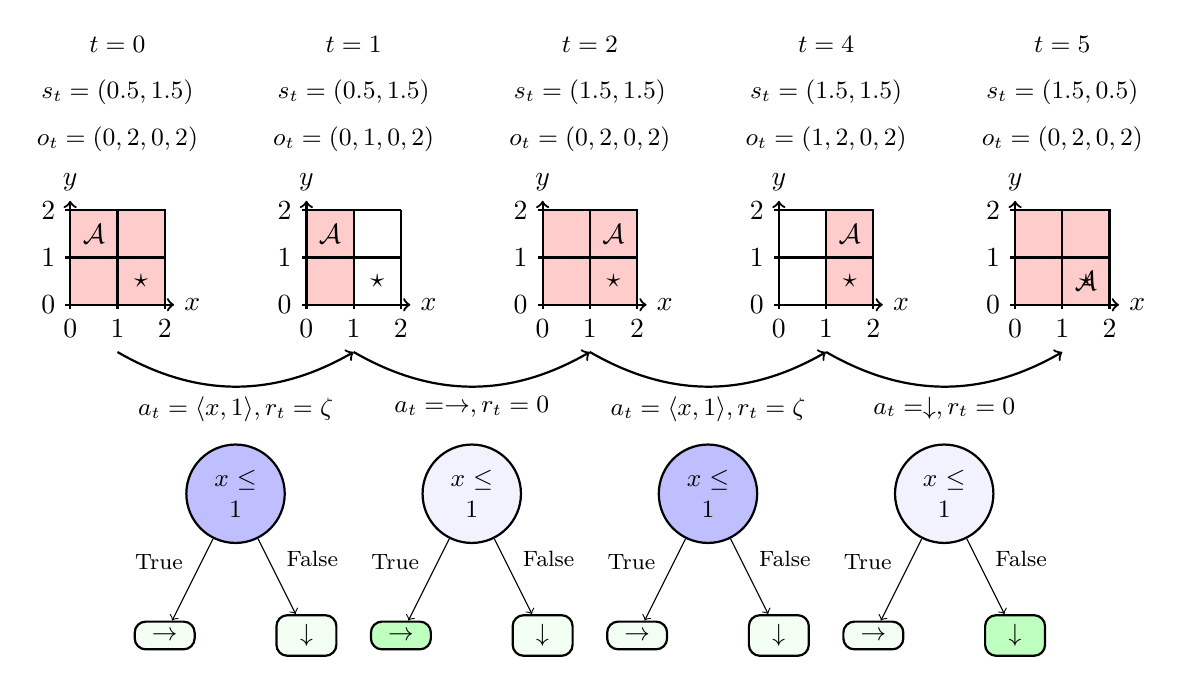
\begin{tikzpicture}[scale=0.6]
    % Define styles
    \tikzstyle{grid}=[draw, thick, fill=gray!10]
    \tikzstyle{rectangle}=[draw, thick, fill=red!20]
    
    % Row 1: IBMDP States (s, o)
    % t=0: Initial state
    \node at (2,9.5) {\small $t=0$};
    \node at (2,8.5) {\small $\boldsymbol{s}_t=(0.5, 1.5)$};
    \node at (2,7.5) {\small $\boldsymbol{o}_t=(0, 2, 0, 2)$};

    \draw[rectangle] (1,4) rectangle (3,6);
    \draw[grid] (1,4) grid (3,6);
    % Add axes
    \draw[thick, ->] (1,4) -- (3.2,4) node[right] {$x$};
    \draw[thick, ->] (1,4) -- (1,6.2) node[above] {$y$};
    \foreach \x in {0,1,2} {
        \draw[thick] (\x+1,4) -- (\x+1,3.9) node[below] {$\x$};
    }
    \foreach \y in {0,1,2} {
        \draw[thick] (1,\y+4) -- (0.9,\y+4) node[left] {$\y$};
    }
    \node at (1.5, 5.5) {$\mathcal{A}$};
    \node at (2.5, 4.5) {$\star$};
    
    % Curved arrow from t=0 to t=1
    \draw[thick, ->] (2,3) to[bend right=30] node[midway, below] {\small $a_t = \langle x, 1\rangle, r_t = \zeta$} (7,3);

    % % t=1: After AIG x≤0.5
    \node at (7,9.5) {\small $t=1$};
    \node at (7,8.5) {\small $\boldsymbol{s}_t=(0.5, 1.5)$};
    \node at (7,7.5) {\small $\boldsymbol{o}_t=(0, 1, 0, 2)$};

    \draw[rectangle] (6,4) rectangle (7,6);
    \draw[grid] (6,4) grid (8,6);
    % Add axes
    \draw[thick, ->] (6,4) -- (8.2,4) node[right] {$x$};
    \draw[thick, ->] (6,4) -- (6,6.2) node[above] {$y$};
    \foreach \x in {0,1,2} {
        \draw[thick] (\x+6,4) -- (\x+6,3.9) node[below] {$\x$};
    }
    \foreach \y in {0,1,2} {
        \draw[thick] (6,\y+4) -- (5.9,\y+4) node[left] {$\y$};
    }
    \node at (6.5, 5.5) {$\mathcal{A}$};
    \node at (7.5, 4.5) {$\star$};


    % Curved arrow from t=1 to t=2
    \draw[thick, ->] (7,3) to[bend right=30] node[midway, below] {\small $a_t = \rightarrow, r_t  = 0$}(12,3);

    \node[circle, draw, thick, fill=blue!25, text width=2em, text centered, minimum height=1.5em, font=\small] (tree4_root) at (4.5,0) {$x \leq 1$};
    \node[rectangle, draw, thick, fill=green!5, text width=1.5em, text centered, rounded corners, minimum height=1em, font=\small] (tree4_right) at (3,-3) {$\rightarrow$};
    \node[rectangle, draw, thick, fill=green!5, text width=1.5em, text centered, rounded corners, minimum height=1em, font=\small] (tree4_left) at (6,-3) {$\downarrow$};
    \draw[->] (tree4_root) -- (tree4_right) node[font=\footnotesize, midway, above left] {True};
    \draw[->] (tree4_root) -- (tree4_left) node[font=\footnotesize, midway, above right] {False};

    \node at (12,9.5) {\small $t=2$};
    \node at (12,8.5) {\small $\boldsymbol{s}_t=(1.5, 1.5)$};
    \node at (12,7.5) {\small $\boldsymbol{o}_t=(0, 2, 0, 2)$};
    
    \draw[rectangle] (11,4) rectangle (13,6);
    \draw[grid] (11,4) grid (13,6);
    % Add axes
    \draw[thick, ->] (11,4) -- (13.2,4) node[right] {$x$};
    \draw[thick, ->] (11,4) -- (11,6.2) node[above] {$y$};
    \foreach \x in {0,1,2} {
        \draw[thick] (\x+11,4) -- (\x+11,3.9) node[below] {$\x$};
    }
    \foreach \y in {0,1,2} {
        \draw[thick] (11,\y+4) -- (10.9,\y+4) node[left] {$\y$};
    }
    \node at (12.5, 5.5) {$\mathcal{A}$};
    \node at (12.5, 4.5) {$\star$};
    
    % Curved arrow from t=2 to t=4
    \draw[thick, ->] (12,3) to[bend right=30] node[midway, below] {\small $a_t = \langle x, 1 \rangle, r_t = \zeta$} (17,3);

    \node[circle, draw, thick, fill=blue!5, text width=2em, text centered, minimum height=1.5em, font=\small] (tree4_root) at (9.5,0) {$x \leq 1$};
    \node[rectangle, draw, thick, fill=green!25, text width=1.5em, text centered, rounded corners, minimum height=1em, font=\small] (tree4_right) at (8,-3) {$\rightarrow$};
    \node[rectangle, draw, thick, fill=green!5, text width=1.5em, text centered, rounded corners, minimum height=1em, font=\small] (tree4_left) at (11,-3) {$\downarrow$};
    \draw[->] (tree4_root) -- (tree4_right) node[font=\footnotesize, midway, above left] {True};
    \draw[->] (tree4_root) -- (tree4_left) node[font=\footnotesize, midway, above right] {False};

    
    \node at (17,9.5) {\small $t=4$};
    \node at (17,8.5) {\small $\boldsymbol{s}_t=(1.5, 1.5)$};
    \node at (17,7.5) {\small $\boldsymbol{o}_t=(1, 2, 0, 2)$};

    \draw[rectangle] (17,4) rectangle (18,6);
    \draw[grid] (16,4) grid (18,6);
    % Add axes
    \draw[thick, ->] (16,4) -- (18.2,4) node[right] {$x$};
    \draw[thick, ->] (16,4) -- (16,6.2) node[above] {$y$};
    \foreach \x in {0,1,2} {
        \draw[thick] (\x+16,4) -- (\x+16,3.9) node[below] {$\x$};
    }
    \foreach \y in {0,1,2} {
        \draw[thick] (16,\y+4) -- (15.9,\y+4) node[left] {$\y$};
    }
    \node at (17.5, 5.5) {$\mathcal{A}$};
    \node at (17.5, 4.5) {$\star$};
    
    \draw[thick, ->] (17,3) to[bend right=30] node[midway, below] {\small $a_t = \downarrow, r_t = 0$} (22,3);
    
    \node[circle, draw, thick, fill=blue!25, text width=2em, text centered, minimum height=1.5em, font=\small] (tree4_root) at (14.5,0) {$x \leq 1$};
    \node[rectangle, draw, thick, fill=green!5, text width=1.5em, text centered, rounded corners, minimum height=1em, font=\small] (tree4_right) at (13,-3) {$\rightarrow$};
    \node[rectangle, draw, thick, fill=green!5, text width=1.5em, text centered, rounded corners, minimum height=1em, font=\small] (tree4_left) at (16,-3) {$\downarrow$};
    \draw[->] (tree4_root) -- (tree4_right) node[font=\footnotesize, midway, above left] {True};
    \draw[->] (tree4_root) -- (tree4_left) node[font=\footnotesize, midway, above right] {False};


    \node at (22,9.5) {\small $t=5$};
    \node at (22,8.5) {\small $\boldsymbol{s}_t=(1.5, 0.5)$};
    \node at (22,7.5) {\small $\boldsymbol{o}_t=(0, 2, 0, 2)$};
 
    \draw[rectangle] (21,4) rectangle (23,6);
    \draw[grid] (21,4) grid (23,6);
    % Add axes
    \draw[thick, ->] (21,4) -- (23.2,4) node[right] {$x$};
    \draw[thick, ->] (21,4) -- (21,6.2) node[above] {$y$};
    \foreach \x in {0,1,2} {
        \draw[thick] (\x+21,4) -- (\x+21,3.9) node[below] {$\x$};
    }
    \foreach \y in {0,1,2} {
        \draw[thick] (21,\y+4) -- (20.9,\y+4) node[left] {$\y$};
    }
    \node at (22.5, 4.5) {$\mathcal{A}$};
    \node at (22.5, 4.5) {$\star$};

    \node[circle, draw, thick, fill=blue!5, text width=2em, text centered, minimum height=1.5em, font=\small] (tree4_root) at (19.5,0) {$x \leq 1$};
    \node[rectangle, draw, thick, fill=green!5, text width=1.5em, text centered, rounded corners, minimum height=1em, font=\small] (tree4_right) at (18,-3) {$\rightarrow$};
    \node[rectangle, draw, thick, fill=green!25, text width=1.5em, text centered, rounded corners, minimum height=1em, font=\small] (tree4_left) at (21,-3) {$\downarrow$};
    \draw[->] (tree4_root) -- (tree4_right) node[font=\footnotesize, midway, above left] {True};
    \draw[->] (tree4_root) -- (tree4_left) node[font=\footnotesize, midway, above right] {False};

    
\end{tikzpicture}}
\caption{Trajectory in an IBMDP of the grid world MDP (\cite{topin2021iterative}). Actions build a decision tree policy and rewards control the interpretability-performance trade-off.}
\end{figure}
\end{frame}

\begin{frame}{Pros and cons of IBMDPs}
\begin{exampleblock}{Pros}
    \begin{itemize}
        \item No need to design new algorithm: we can use deep RL.
        \item IBMDP rewards trade-off naturally interpretability and performances.
    \end{itemize}
\end{exampleblock}
\begin{alertblock}{Cons}
    \begin{itemize}
        \item Only \textbf{determinstic} and \textbf{partially observable} (a.k.a. memoryless or reactive) policies are equivalent to decision tree policies.
        \item Finding the best \textbf{deterministic} and \textbf{partially observable} policy is NP-hard (\cite{littman1})!
    \end{itemize}
\end{alertblock}
\end{frame}

\begin{frame}{Re-formulation}
    \textit{Q: Can we use reinforcement learning to directly optimize trade-offs of performance and interpretability in SDM?} $\Leftrightarrow$ \\
    \textit{Q: How does RL perform for optimizing \textbf{deterministic} and \textbf{partially observable} policies in IBMDPs?
}
\end{frame}

\begin{frame}{Result: RL cannot retrieve optimal depth-1 trees for the grid world MDP}
\begin{figure}
    \centering
    \includegraphics[width=1\textwidth]{../images/images_part1/tree_distributions.pdf}
    \caption{Distributions of final tree policies learned with various (asymmetric) RL algorithms (\cite{sutton,learning-pomdp,sarsa-pomdp,baisero-ppo,baisero-dqn}) across 100 seeds.
    For each different performance-interpretability trade-off value $\zeta$, each point represent the share of different trees.
    }
\end{figure}
\end{frame}

\begin{frame}{Result: for similar problems, RL struggles when there is partial observability (not surprising)}
\begin{figure}
    \centering
    \includegraphics[width=0.65\textwidth]{../images/images_part1/algorithm_performance_comparison_flattened.pdf}
    \caption{Success rates of different (asymmetric) RL algorithms over thousands of runs when applied to learning either deterministic partially observable policies in an IBMDP deterministic Markovian policies in the same IBMDP.}
\end{figure}
\end{frame}

\begin{frame}{Interesting sub-class of MDPs: classification MDPs}
\begin{figure}
    \centering
    \begin{tikzpicture}[
        decision/.style={circle, draw, thick, fill=blue!20, text width=2.5em, text centered, minimum height=2.5em, font=\small},
        leaf/.style={rectangle, draw, thick, fill=green!20, text width=2em, text centered, rounded corners, minimum height=2em, font=\small},
        edge_label/.style={font=\footnotesize, midway}
    ]
        % Tree 4: if x <= 0.5 move right else move left
        \node[decision] (tree4_root) at (8,2) {$x \leq 1$};
        \node[rectangle, draw, thick, fill=green!40, text width=2em, text centered, rounded corners, minimum height=2em, font=\small] (tree4_right) at (7,0) {};
        \node[rectangle, draw, thick, fill=red!40, text width=2em, text centered, rounded corners, minimum height=2em, font=\small] (tree4_left) at (9,0);
        \draw[->] (tree4_root) -- (tree4_right) node[edge_label, above left] {True};
        \draw[->] (tree4_root) -- (tree4_left) node[edge_label, above right] {False};
        \tikzstyle{grid}=[draw, thick, fill=gray!10]
        
        % Draw grid
        \draw[fill=green!40] (0, 0) rectangle (1,2);
        \draw[fill=red!40] (1, 0) rectangle (2,2);

        \draw[grid] (0,0) grid (2,2);
        
        % Add axes
        \draw[thick, ->] (0,0) -- (2.5,0) node[right] {$x$};
        \draw[thick, ->] (0,0) -- (0,2.5) node[above] {$y$};
        
        % Add tick marks and labels
        \foreach \x in {0,1,2} {
            \draw[thick] (\x,0) -- (\x,-0.1) node[below] {$\x$};
        }
        \foreach \y in {0,1,2} {
            \draw[thick] (0,\y) -- (-0.1,\y) node[left] {$\y$};
        }

        \node at (0.5,0.5) {$\boldsymbol{s}_0$};
        \node at (1.5,0.5) {$\boldsymbol{s}_g$};
        \node at (1.5,1.5) {$\boldsymbol{s}_2$};
        \node at (0.5,1.5) {$\boldsymbol{s}_1$};

    \end{tikzpicture}
    \caption{In this classification MDP, there are four data to which to assign either a green or red label.
    On the right, there is the unique optimal depth-1 tree for this particular classification MDP.}
    \textbf{We show that in theory, deterministic partially observable policies for classification IBMDPs ($\Leftrightarrow$ decision tree policies) are in fact Markovian.}    
\end{figure}
\end{frame}

% \begin{frame}{Experimental result: for SDM problems $\Leftrightarrow$ classification problems, RL can consistently retrieve optimal depth-1 decision tree policies}
% \begin{figure}
%     \centering
%     \includegraphics[width=1\textwidth]{../images/images_part1/tree_distributions_classif.pdf}
%     \caption{Each colored dot is the number of final learned trees with a specific structure for a given $\zeta$. Those results makes sense because we can show that IBMDPs for classification tasks don't have a partial observability component.}\label{fig:tree-distrib-classif-poibmdp}
% \end{figure}
% \end{frame}

\begin{frame}{Perspectives for direct RL of decision tree policies.}
    \begin{itemize}
        \item Learning decision tree policies that trade-off performances and interpretability for SDM problems is difficult because for most problems there is \textcolor{red}{partial observability}.
        \item Should we focus on indirect approach? There is a potential for hybrid approaches (\cite{parbhoo})
        \item What are the pros and cons of fixing the policy tree structure a priori (paramteric trees, \cite{sympol})?
        \item Can we specifically design algorithms that learn deterministic partially observable policies (\cite{lambrechts2025informed,justif-asym})?
    \end{itemize}
    \begin{exampleblock}{RL works in classification MDPs}
    \textit{Q: Can we leverage SDM in classification MDPs to design new decision tree induction algorithms for the supervised learning (no sequentiality) setting?}
    \textbf{A: Yes!}
    \end{exampleblock}
\end{frame}

\begin{frame}{Decision trees in supervised learning}
\begin{itemize}
    \item We assume that we have access to a set of $N$ examples denoted $\mathcal{E} = {\{(x_i, y_i)\}}_{i=1}^N$. Each datum $x_i$ is described by a set of $p$ features. $y_i \in {\mathcal Y}$ is the label associated with $x_i$.
    \begin{align}
        \mathcal{L}(T) = \frac{1}{N}\overset{N}{\underset{i=1}{\sum}}{\ell}(y_i, f(x_i)) + \alpha C(T)
    \end{align}
    where $C: \mathcal{\mathcal{T}} \rightarrow \mathbb{R}$ is a penalty for tree interpretability/regularization.
    \item Tree-based models perform really well on \textbf{tabular} data, often \textbf{better than deep neural nets} (\cite{grinsztajn2022tree}).
\end{itemize}
\end{frame}

\begin{frame}{Optimal decision tree induction is NP-hard}
\begin{itemize}
    \item Greedy algorithms (\cite{breiman1984classification,ID3,c45}) \textcolor{red}{sub-optimal accuracy}, but time complexity in \textcolor{green}{$O(2^D)$}.
    \item Optimal algorithms (\cite{oct,murtree,pystreed,chaouki2024branchesfastdynamicprogramming}), \dots) \textcolor{green}{optimal accuracy}, but time complexity in \textcolor{red}{$O((2Np)^D)$}.
\end{itemize}
\end{frame}

\begin{frame}{In between?}
    \begin{figure}
        \centering
        \includegraphics[width=1\linewidth]{../images/figures/patho_bounds_comparison_checkers.pdf}
        \caption{A checkers board data set highlights the limitations of existing works.}
    \end{figure}
\end{frame}

\begin{frame}{Decision tree induction as solving MDPs}

\begin{block}{Intuition}
    Given a set of examples $\mathcal{E}$, the induction of a decision tree is made of a sequence of decisions: at each node, we must decide whether it is better to split (a subset of) $\mathcal{E}$, or %assign a class label and 
    to create a leaf node.
\end{block}
\begin{itemize}
    \item S: data subsets.
    \item A: test or leaf nodes that can be added to the tree.
    \item R: penalty or accuracies.
    \item T: node traversals.
\end{itemize}
\end{frame}

\begin{frame}{Decision tree induction as solving MDPs}
\begin{figure}
    \centering
    \includegraphics[width=1\linewidth]{../images/figures/schema_mdp.pdf}
    \caption{MDP formulation of a generic decision tree induction for a supervised learning task.}
\end{figure}
\end{frame}

% \begin{frame}{Objective Leftrightarrowalence}
% \begin{block}{Objective Equivalence}\label{prop:Leftrightarrow}
% Let $\pi$ be a deterministic policy of the MDP and $\pi^*$ be an optimal deterministic policy. 
% Then $J_\alpha(\pi) = -{\mathcal L}_\alpha(E(\pi, s_0))$ and $T^* = E(\pi^*, s_0)$ where $T^*$ is a tree that optimizes Eq.~\ref{eq:suplearning}.
% \end{block}
% \begin{alertblock}{Interpretation}
% We can learn a decision tree that maximizes accuracy by finding an MDP policy that maximizes rewards (this can be done easily with DP).
% \end{alertblock}
% \end{frame}
\begin{frame}{Controlling the time complexity of decision tree induction}

\begin{itemize}
    \item Greedy algorithms consider only one candidate action in each state which is the test that minimizes some impurity criterion $\rightarrow$ \textcolor{green}{MDP state space size is $O(2^D)$}.
    \item Optimal algorithms consider all possible actions in each state $\rightarrow$ \textcolor{red}{MDP state space size is $O((2Np)^D)$}.
    \item Let's choose candidate actions adaptively $\rightarrow$ for each MDP state consider $B$ actions: \textcolor{blue}{state space size is $O((2B)^D)$}.
\end{itemize}
\end{frame}

\begin{frame}{Dynamic Programming Decision Trees (DPDT)\footnote{Because states are entire datasets, we implement DPDT with a depth-first search to limit the space complexity.}}
\begin{figure}
    \centering
    \includegraphics[width=0.7\linewidth]{../images/figures/schematic_cart_node_select.pdf}
    \caption{Overview of our algorithm DPDT presented at the 31st ACM SIGKDD conference.}
\end{figure}
\end{frame}

\begin{frame}{Comparing tree accuracy to complexity}
\begin{table}
    \caption{Train accuracy and operation count when learning depth-3 decision trees.}
    \tiny
    \begin{tabular}{l|cc||cc|cc|c||cc|cc}
    \toprule
    & & & \multicolumn{5}{c||}{\textbf{Accuracy}} & \multicolumn{4}{c}{\textbf{Operations}}\\
    \midrule
    & & & Opt & Greedy & \multicolumn{2}{c|}{DPDT} & \multicolumn{1}{c||}{} & Opt & Greedy & \multicolumn{2}{c|}{DPDT}\\
    \textbf{Dataset} & N & p & Quant-BnB & CART & light & full & & Quant-BnB & CART & light & full \\
    \midrule
    room & 8103 & 16 & \textbf{0.992} & 0.968 & \color{blue} 0.991 & \textbf{0.992} & &$10^6$ & 15 & 286 & 16100 \\
    bean & 10888 & 16  & \textbf{0.871} & 0.777 & 0.812 & \color{blue} 0.853 & & 5$\cdot 10^6$ & 15 & 295 & 25900 \\
    eeg & 11984 & 14  & \textbf{0.708} & 0.666 & 0.689 & \color{blue} 0.706 & & 2$\cdot 10^6$ & 13 & 289 & 26000 \\
    avila & 10430 & 10  & \textbf{0.585} & 0.532 & \color{blue}0.574 & \textbf{0.585} & & 3$\cdot 10^7$ & 9 & 268 & 24700 \\
    magic & 15216 & 10 & \textbf{0.831} & 0.801 & 0.822 & \color{blue} 0.828 & &6$\cdot 10^6$ & 15 & 298 & 28000 \\
    htru & 14318 & 8  & \textbf{0.981} & 0.979 & 0.979 & \color{blue}0.980 & & 6$\cdot 10^7$ & 15 & 295 & 25300 \\
    occup. & 8143 & 5 & \textbf{0.994} & 0.989 & 0.991 & \textbf{0.994} & & 7$\cdot 10^5$ & 13 & 280 & 16300 \\
    skin & 196045 & 3 & \textbf{0.969} & \color{blue}0.966 & \color{blue}0.966 & \color{blue}0.966 & & 7$\cdot 10^4$ & 15 & 301 & 23300 \\
    fault & 1552 & 27 & \textbf{0.682} & 0.553 & 0.672 & \color{blue}0.674 & & 9$\cdot 10^8$ & 13 & 295 & 24200 \\
    segment & 1848 & 18 & \textbf{0.887} & 0.574 & 0.812 & \color{blue}0.879 & & 2$\cdot 10^6$ & 7 & 220 & 16300 \\
    page & 4378 & 10 &  \textbf{0.971} & 0.964 & \color{blue}0.970 & \color{blue}0.970 & &$10^7$ & 15 & 298 & 22400 \\
    bidding & 5056 & 9  & \textbf{0.993} & 0.981 & \color{blue}0.985 & \textbf{0.993} & & 3$\cdot 10^5$ & 13 & 256 & 9360 \\
    raisin & 720 & 7 & \textbf{0.894} & 0.869 & 0.879 & \color{blue}0.886 & & 4$\cdot 10^6$ & 15 & 295 & 20900 \\
    rice & 3048 & 7 & \textbf{0.938} & 0.933 & 0.934 & \color{blue}0.937 & & 2$\cdot 10^7$ & 15 & 298 & 25500 \\
    wilt & 4339 & 5 & \textbf{0.996} & 0.993 & 0.994 & \color{blue}0.995 & &3$\cdot 10^5$ & 13 & 274 & 11300 \\
    bank & 1097 & 4 & \textbf{0.983} & 0.933 & 0.971 & \color{blue}0.980 & & 6$\cdot 10^4$ & 13 & 271 & 7990 \\
    \bottomrule
    \end{tabular}
\end{table}
\end{frame}

\begin{frame}{DPDT trees generalization}
    \begin{figure}
     \centering
     \begin{subfigure}[b]{0.32\textwidth}
         \centering
         \includegraphics[width=\textwidth]{../images/figures/tab_bench/random_search_classif_numerical_depth5.pdf}
         \caption{DPDT depth-5 trees vs. other detph-5 trees}
     \end{subfigure}
     \hfill
     \begin{subfigure}[b]{0.32\textwidth}
         \centering
         \includegraphics[width=\textwidth]{../images/figures/tab_bench/random_search_classif_categorical_boosting_w_weak.pdf}
         \caption{Boosted DPDT vs. Boosted CART}
     \end{subfigure}
     \hfill
     \begin{subfigure}[b]{0.32\textwidth}
         \centering
         \includegraphics[width=\textwidth]{../images/figures/tab_bench/random_search_classif_numerical_boosting_all_notgb.pdf}
         \caption{Boosted DPDT vs. other classifiers}
     \end{subfigure}
\end{figure}
\end{frame}

\begin{frame}{Perspectives}
    \begin{itemize}
        \item New SOTA decision tree induction with dynamic programming in MDPs.
        \item What about using DPDT for indirect decision tree policy learning for SDM?
        \item What performances could we reach with an industry-grade implementation of XGboost+DPDT?
    \end{itemize}
    \begin{exampleblock}{Let us take a step back}
        \textit{Q: Are decision trees really the most interpretable model?}\\
        \textbf{A: It depends.}
    \end{exampleblock}
\end{frame}


\begin{frame}{How to measure policy interpretability?}
\begin{alertblock}{Challenges (\cite{glanois-survey,lipton,rigourous})}
\begin{itemize}
    \item There is no clear definition of interpretability.
    \item Measuring interpretability might require humans.
\end{itemize}
\end{alertblock}

\begin{exampleblock}{The notion of \textit{simulatability} (\cite{lipton})}
\begin{itemize}
    \item Interpretability $\simeq$ how long it takes for human to make the same computations given an input.
    \item Interpretability $\simeq$ how much effort it would take a human to read through the entire policy once.
    \item Inside a given policy class, less parameters should mean more interpretability (\cite{study-0,study-4,study-5,study-6,study-7}).
    \item The time required to formally verify a policy should decrease with interpretability (\cite{viper,lens-complexity}).
\end{itemize}
\end{exampleblock}
\end{frame}

\begin{frame}{A methodology to measure policy interpretability without humans}
\begin{block}{Simulatability (\cite{lipton})}
\begin{enumerate}
    \item How long it takes for human to make the same computations given an input $\simeq$ policy inference time.
    \item How much effort it would take a human to read through the entire policy once $\simeq$ policy size in memory.
\end{enumerate}
\end{block}
\begin{alertblock}{Not that simple in practice (\cite{insight})}
\begin{itemize}
    \item Different hardwares (tree policies are run on CPUs while neural policies are run on GPUs).
    \item Different implementations (neural policies compute outputs using matrix operations while tree operate fully sequentially) $\dots$
\end{itemize}
\end{alertblock}
\end{frame}

\begin{frame}[fragile]{We propose policy unfolding}
\begin{minipage}{0.48\textwidth}
\begin{tcolorbox}
\begin{lstlisting}[language=Python]
# Decision tree for Mountain Car
def play(x):
    if x[1] <= -0.2597:
        if x[1] <= -0.6378:
            return 0
        else:
            if x[0] <= -1.0021:
                return 2
            else:
                return 0
    else:
        if x[1] <= -0.0508:
            if x[0] <= 0.2979:
                if x[0] <= 0.0453:
                    return 2
                else:
                    if x[1] <= -0.2156:
                        return 0
                    else:
                        return 2
            else:
                return 0
        else:
            return 2
\end{lstlisting}
\end{tcolorbox}
\end{minipage}
\hfill
\begin{minipage}{0.5\textwidth}
\begin{tcolorbox}
\begin{lstlisting}[language=Python]
# Small ReLU MLP for Pendulum
def play(x):
    h_layer_0_0 = 1.238*x[0]+0.971*x[1]
                  +0.430*x[2]+0.933
    h_layer_0_0 = max(0, h_layer_0_0)
    h_layer_0_1 = -1.221*x[0]+1.001
                  *x[1]-0.423*x[2]
                  +0.475
    h_layer_0_1 = max(0, h_layer_0_1)
    h_layer_1_0 = -0.109*h_layer_0_0
                  -0.377*h_layer_0_1
                  +1.694
    h_layer_1_0 = max(0, h_layer_1_0)
    h_layer_1_1 = -3.024*h_layer_0_0
                  -1.421*h_layer_0_1
                  +1.530
    h_layer_1_1 = max(0, h_layer_1_1)

    h_layer_2_0 = -1.790*h_layer_1_0
                  +2.840*h_layer_1_1
                  +0.658
    y_0 = h_layer_2_0
    return [y_0]
\end{lstlisting}
\end{tcolorbox}
\end{minipage}
\end{frame}

\begin{frame}{Empirical validation}
\begin{enumerate}
    \item Does our methodology respect consensus on policy interpretability?
    \item Is policy unfolding necessary to respect the consensus?
    \item What kind of results we can obtain using our proposed methodology?
\end{enumerate}
\\
We imitate $\sim40000$ expert policies from \texttt{stable-baselines3} using various policy classes/nb parameters on various environments.
\end{frame}


% \begin{frame}{Empirical validation: obtaining $\sim40000$ policies from different classes}
% \begin{table}[ht]
% \hspace{-0.3cm}
% \centering
% \footnotesize
% \begin{tabular}{lll}
% \hline
% \textbf{Policy Class} & \textbf{Parameters} & \textbf{Training algo.} \\
% \hline
% Linear policies & Determined by state-action dimensions & Linear/logistic Reg. \\
% Decision trees & \{4, 8, 16, 64, 128\} nodes & CART \\
% Oblique decision trees & \{4, 8, 16, 64, 128\} nodes & CART \\
% Relu neural networks & \{(2 ,2), (4, 4), (8, 8), (16, 16)\} weights & SGD \\
% \hline
% \end{tabular}
% \caption{Summary of policy classes parameters and supervised learning algorithms to fit experts.}
% \end{table}
% \end{frame}

% \begin{frame}{Empirical validation: obtaining $\sim40000$ policies from different classes}

% \begin{table}[ht]
% \hspace{-0.48cm}
%   \centering
%   \footnotesize
%   \begin{tabular}{lll}
%   \hline
%   \textbf{Classic} & \textbf{MuJoCo} & \textbf{OCAtari}\\
%   \hline
%   CartPole (4, 2, \textbf{490}) & Swimmer (8, 2, \textbf{300}) & Breakout (452, 4, \textbf{30})\\
%   LunarLander (8, 4, \textbf{200}) & Walker2d (17, 6, \textbf{2000}) & Pong (20, 6, \textbf{14})\\
%   //    Continuous (8, 2, \textbf{200}) & HalfCheetah (17, 6, \textbf{3000}) & SpaceInvaders (188, 6, \textbf{680})\\
%   BipedalWalker (24, 4, \textbf{250}) & Hopper (11, 3, \textbf{2000}) & Seaquest (180, 18, \textbf{2000})\\
%   MountainCar (2, 3, \textbf{90}) & \\
%   //    Continuous (2, 1, \textbf{-110}) & \\
%   Acrobot (6, 3, \textbf{-100}) & \\
%   Pendulum (3, 1, \textbf{-400}) & \\
%   \hline
%   \end{tabular}
%   \caption{Summary of considered environments (dimensions of states and number or dimensions of actions, \textbf{performance thresholds to solve}). OCAtari is an object-centric version of Atari.}
%   \end{table}

% \end{frame}

\begin{frame}{Result: unfolding policies is necessary to respect consensus}
\begin{figure}
    \centering
    \includegraphics[width=1\linewidth]{../images/images_part3/tree_sizes_memory_ppo_ci_ablation.pdf}
    \caption{Policies interpretability on classic control environments. We plot 95\% stratified bootstrapped confidence intervals around means in both axes. In each sub-plot, interpretability is measured with either bytes or inference speed.}
    \label{fig:abl-proxies}
\end{figure}
\end{frame}


% \begin{frame}{Result: verification time does scale with step inference time}
%     \begin{figure}[ht]
%     \centering
%     \includegraphics[width=1\linewidth]{../images/images_part3/verification_tradeoff.pdf}
%     \caption{Verification time as a function of policy interpretability. Top row, interpretability is measured with step inference times. Bottom row, the interpretability is measured with policy size.}
%     \label{fig:trade-off-verif}
% \end{figure}
% \end{frame}

\begin{frame}{Result: there is no dominating policy class for all environments}
\begin{figure}
    \centering
    \includegraphics[trim={1.4cm 0 0 0},clip,width=1\textwidth]{../images/images_part3/trade_off_select_combine_one_plot.pdf}
    \caption{Interpretability-Performance trade-offs for representative environments. Top row, interpretability is measured with step inference times. Bottom row, the interpretability is measured with policy size.}
    \label{fig:trade-off-summary}
\end{figure}
\end{frame}

\begin{frame}{Perspectives}
\begin{itemize}
    \item Because there is no dominating class for all problems in terms of interpretability-performance trade-offs, beliefs such as "trees are more interpretable than neural networks" should be used with caution.
    \item Tree-like policy classes can have good inductive bias for game-like envrionments.
    \item Can a human study confirm our results?
    \item Can our methodology be used for evaluating the interpretability of (very) big models?
    \item Can we use our policy programs as low level skills (hierarchical RL)? 
\end{itemize}
\end{frame}

\begin{frame}{Conclusion: interpretable machine learning is a difficult research topic}
    \begin{itemize}
        \item Technical challenges: \textcolor{red}{partial observability in SDM, NP-hardness}.\\ $\rightarrow$ Focus on indirect approaches and/or on POMDP research first.
        \item Fundamental challenges: \textcolor{red}{no definition}. \\ $\rightarrow$ Discuss with the community (\underline{InterpPol workshop}).
        \item \textcolor{green}{Decision trees offer good inductive bias for SDM in games or tabular data}.
    \end{itemize}
    \begin{block}{My hope}
        Motivate interpretability by finding a real-world problem where interpretability is \textit{really} necessary (\cite{festor}).
    \end{block}
\end{frame}

\printbibliography
\end{document}